\section{Podzadanie B}
\subsection{Rozkład danych}
\subsubsection{Rozkład wartości etykiet}

Podzadanie B miało na celu określenie podobieństwa pomiędzy istniejącym a nowym pytaniem. Pytania posiadały trzy etykiety określające stopień podobieństwa: ,,PerfectMatch'', ,,Relevant'' i ,,Irrelevant''. Rozkład etykiet w oryginalnym zbiorze został przedstawiony w tablicy 5.9.

\begin{table}[H]
\caption{Rozkład klas w oryginalnym zbiorze}
\label{subtask_b_original_set_statistics_score_table}
    \begin{center}
        \begin{tabular}{ |c|c| } 
            \hline
            ,,PerfectMatch'' & 9,28\% \\
            \hline
            ,,Relevant'' & 31,65\% \\
            \hline
            ,,Irrelevant'' & 59,07\% \\ 
            \hline
        \end{tabular}
    \end{center}
\end{table}

Etykiety ,,PerfectMatch'' i ,,Relevant'' zostały określane jako równoważne, w związku z czym zredukowano liczbę etykiet do dwóch, o następujących nazwach: ,,Relevant'' i ,,Irrelevant''. Dodatkowo, cały zbiór podzielono losowo na podzbiór treningowy i walidujący w proporcjach 4:1. Tablice 5.10 oraz 5.11 przedstawiają rozkład klas w utworzonych podzbiorach.

\begin{table}[H]
\caption{Rozkład klas w zbiorze treningowym.}
\label{subtask_b_train_set_statistics_score_table}
    \begin{center}
        \begin{tabular}{ |c|c| } 
            \hline
            ,,Relevant'' & 40,83\% \\
            \hline
            ,,Irrelevant'' & 59,17\% \\ 
            \hline
        \end{tabular}
    \end{center}
\end{table}

\begin{table}[H]
\caption{Rozkład klas w zbiorze treningowym.}
\label{subtask_b_validation_set_statistics_score_table}
    \begin{center}
        \begin{tabular}{ |c|c| } 
            \hline
            ,,Relevant'' & 41,33\% \\
            \hline
            ,,Irrelevant'' & 58,67\% \\ 
            \hline
        \end{tabular}
    \end{center}
\end{table}

Liczność etykiet różni się minimalnie pomiędzy wydzielonymi pozbiorami. W obu można zauważyć przewagę liczności etykiet ,,Irrelevant'' nad etykietami ,,Relevant'', jednak ciężko stwierdzić, aby doszło znacznej skośności danych.

\subsection{Analiza danych}

W ramach wstępnej analizy danych i zdobycia poglądowej wiedzy na temat zbioru danych wykonane zostały obliczenia powszechnych miar statystycznych stosowanych w przetwarzaniu języka naturalnego takich jak: indeks Jaccarda, podobieństwo kosinusowe oraz różnica długości tekstu. Następnie wyniki przedstawiono z podziałem na rodzaj etykiety (rysunek~\ref{fig:lenghtb}).

\begin{figure}[H]
\caption{Zależność różnicy długości i etykiety.\label{fig:lenghtb}}
\centering
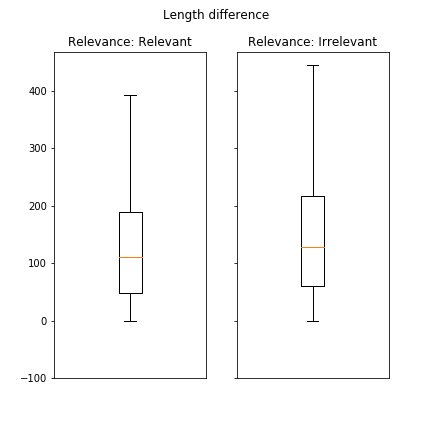
\includegraphics[scale=0.5]{subtask_b_length_difference.png}
\end{figure}

Dla pytań z etykietą ,,Relevant'' wartości maksymalne oraz mediana są mniejsze od pytań z etykietą ,,Irrelevant''. Poza tym, nie występują inne znaczące różnice.

\begin{figure}[H]
\caption{Zależność odległości Jaccarda i etykiety. \label{fig:Jaccardb}}
\centering
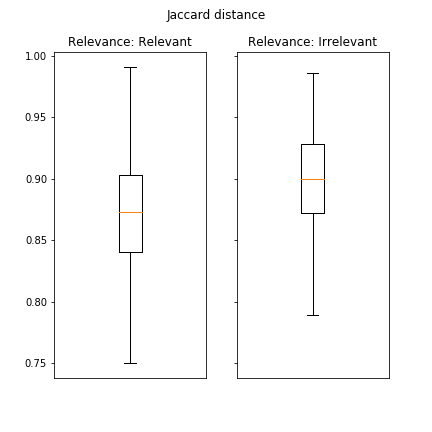
\includegraphics[scale=0.5]{subtask_b_jaccard_distance.png}
\end{figure}

W przypadku odległości Jaccarda pytania z etykietą Relevant uzyskiwały mniejsze wartości mediany (rysunek~\ref{fig:Jaccardb}). Prawie połowa rezultatów zawarła się w zakresie od 0,85 do 0,90, gdzie dla pytań ,,Irrelevant'' były to wartości od 0,88 do 0,93.

\begin{figure}[H]
\caption{Zależność podobieństwa kosinusowego i etykiety. \label{fig:cosinusb}}
\centering
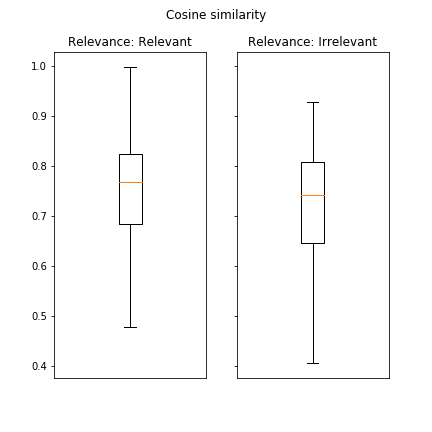
\includegraphics[scale=0.5]{subtask_b_cosine_similarity.png}
\end{figure}

W ostatnim przypadku obliczono podobieństwo kosinusowe i tak jak w przypadku poprzednich miar nie zauważono wyraźnej zależności pomiędzy etykietą a wynikami. Mediana dla ,,Relevant'' była nieznacznie większa od mediany ,,Irrelevant'' (rysunek~\ref{fig:cosinusb}).


\subsection{Sieć rekurencyjna}
\subsubsection{Rezultaty dla pierwotnego zbioru danych}

Aby umożliwić wydajną naukę sieci neuronowej, dane zostały przetworzone do nowego formatu. Oryginalnie pytanie było podzielone na tytuł i korpus. Okazało się jednak, że korpus często zawierał powtórzone pytanie. Stąd decyzja o odrzuceniu tytułu i reprezentowaniu pytania wyłącznie przez korpus. Ponieważ zadaniem była klasyfikacja binarna, zamiast etykiet ,,Relevant'' i ,,Irrelevant'', utworzono jedną etykietę o nazwie ,,Relevance'', która przyjmowała wartość 0 dla ,,Irrelevant'' i 1 dla ,,Relevant''.

Wykorzystana sieć neuronowa była siecią syjamską. Posiadała dwa wejścia, każde z nich przyjmowało wektor indeksów słów występujących w zbiorze treningowym. W kolejnej warstwie elementy wektora wejściowego były przekształcane do word-embeddingów. Następnie użyta została warstwa rekurencyjna, gdzie oba pytania były przetwarzane osobno. Rezultaty zostały porównane w ostatniej warstwie, w oparciu o odległość manhattańską. Wynikiem była liczba z zakresu [0,1]. Para pytań uznawana była za podobną gdy otrzymano wartość większą od 0,5.

Do uczenia sieci użyto całego zbioru treningowego składającego się z 2499 par pytań, z czego 250 elementów wyodrębnione zostało do zbioru walidującego.

\begin{figure}[H]
\caption{Skuteczność sieci syjamskiej.\label{fig:suktecznoscbacc}}
\centering
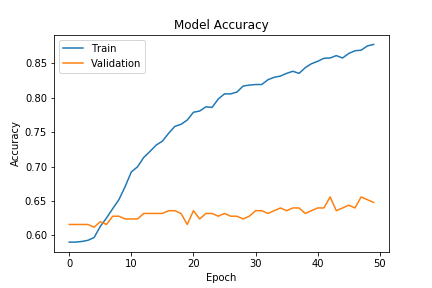
\includegraphics[scale=0.7]{subtask_b_first_gen_model_accuracy.png}
\end{figure}

\begin{figure}[H]
\caption{Strata sieci syjamskiej.\label{fig:suktecznoscbloss}}
\centering
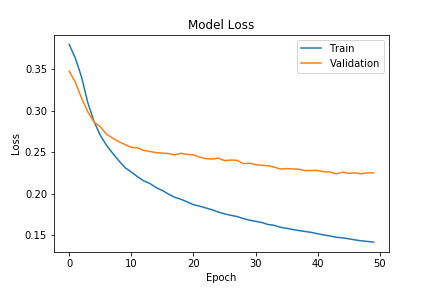
\includegraphics[scale=0.7]{subtask_b_first_gen_model_loss.png}
\end{figure}

Na powyższych wykresach (rysunki~\ref{fig:suktecznoscbacc} i \ref{fig:suktecznoscbloss}) widać, że po kilkunastu epokach doszło do przeuczenia sieci. W kolejnych epokach rosła dokładność na zbiorze treningowym, a dla zbioru walidującego utrzymywała się na tym samym poziomie. Ponieważ dokładność nie prezentuje pełnych informacji na temat wyuczonego modelu, w tablicy~\ref{tab:train_set_statistics_score_tableb}  przedstawione zostały jeszcze następujące miary: pokrycia, krzywa ROC (ang. \textit{Receiver operating characteristic}) i błędu pierwszego stopnia (ang. \textit{F1 score}).

\begin{table}[H]
\caption{Skuteczność sieci rekurencyjnej na zbiorze testowym.}
\label{tab:train_set_statistics_score_tableb}
    \begin{center}
        \begin{tabular}{ |c|c| } 
            \hline
            metryka & wartość\\
            \hline
            Accuracy & 0,639 \\
            \hline
            Precision & 0,312 \\
            \hline
            Recall & 0,625 \\ 
            \hline
            ROC curve & 0,634 \\ 
            \hline
            F1 score & 0,417 \\ 
            \hline
        \end{tabular}
    \end{center}
\end{table}

\subsubsection{Rezultaty dla rozszerzonego zbioru danych}

Jednym z najlepszych sposobów na pozyskanie lepszych wyników jest często zebranie większej ilości danych. W tym celu można skorzystać z innych, otwartych zbiorów danych w internecie. Niestety, takie zbiory mogą różnić się jakością i ostatecznie doprowadzić do pogorszenia wyników, dlatego zastosowano alternatywne podjeście. Kolejne pary były generowane dzięki zaobserwowaniu prostej zależności: nowe pytania o identycznej skali podobieństwa względem istniejącego pytania i występujące we wspólnym wątku powinny utworzyć nową parę o takiej samej istotności.
Zmodyfikowane zbiory miały następujący rozkład klas:

\begin{table}[H]
\caption{Rozkład klas w rozszerzonym zbiorze treningowym.}
\label{subtask_b_original_set_statistics_score_table}
    \begin{center}
        \begin{tabular}{ |c|c| } 
            \hline
            ,,Relevant'' & 31,55\% \\
            \hline
            ,,Irrelevant'' & 68,45\% \\ 
            \hline
        \end{tabular}
    \end{center}
\end{table}

\begin{table}[H]
\caption{Rozkład klas w rozszerzonym zbiorze testowym.}
\label{subtask_b_original_set_statistics_score_table}
    \begin{center}
        \begin{tabular}{ |c|c| } 
            \hline
            ,,Relevant'' & 30,48\% \\
            \hline
            ,,Irrelevant'' & 69,52\% \\ 
            \hline
        \end{tabular}
    \end{center}
\end{table}

Zachowane zostały proporcje klas, nadal najwięcej jest par o niskim podobieństwie.
Zbiór treningowy składał się z 9000, a testowy z 2395 par pytań.

\begin{figure}[H]
\caption{Skuteczność sieci syjamskiej po rozszerzeniu zbioru danych.}
\centering
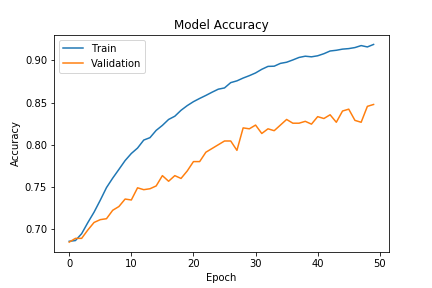
\includegraphics[scale=0.7]{subtask_b_second_gen_model_accuracy.png}
\end{figure}

\begin{figure}[H]
\caption{Strata sieci syjamskiej po rozszerzeniu zbioru danych.}
\centering
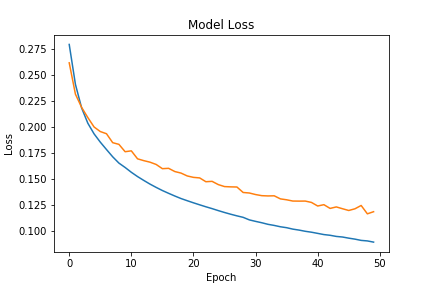
\includegraphics[scale=0.7]{subtask_b_second_gen_model_loss.png}
\end{figure}

\begin{table}[H]
\caption{Skuteczność sieci rekurencyjnej na zbiorze testowym.}
\label{train_set_statistics_score_table}
    \begin{center}
        \begin{tabular}{ |c|c| } 
            \hline
            metryka & wartość\\
            \hline
            Accuracy & 0,846 \\
            \hline
            Precision & 0,838 \\
            \hline
            Recall & 0,699 \\ 
            \hline
            ROC curve & 0,824 \\ 
            \hline
            F1 score & 0,771 \\ 
            \hline
        \end{tabular}
    \end{center}
\end{table}

\subsection{Ocena rezultatów}
Analizując wyniki otrzymane po wyuczeniu sieci syjamskich można stwierdzić, że rozszerzenie zbioru danych miało pozytywny wpływ na jakość klasyfikatora. Stworzenie nowych przykładów uczących zmieniło co prawda rozkład klas w zbiorze treningowym dla ,,Relevant'' z 40,8\% na 31,5\% i ,,Irrelevant'' z 59,2\% na 68,5\%, jednakże w tym samym czasie zaobserwowano wzrost m.in. dokładności sieci z 63,9\% na 84,6\%. 
